\chapter{Running Map/Reduce in a multi-node cluster}
\par In this section we will running a Map / Reduce program in a multi-node cluster.
%Intro\footnotemark\\
\begin{spacing}{1.2}
%note en bas de page
\section{Checking all the nodes of the cluster}

\par Let's verify the good functioning of all the nodes of the cluster.
\\
\begin{figure}[!htb] 
\begin{center} 
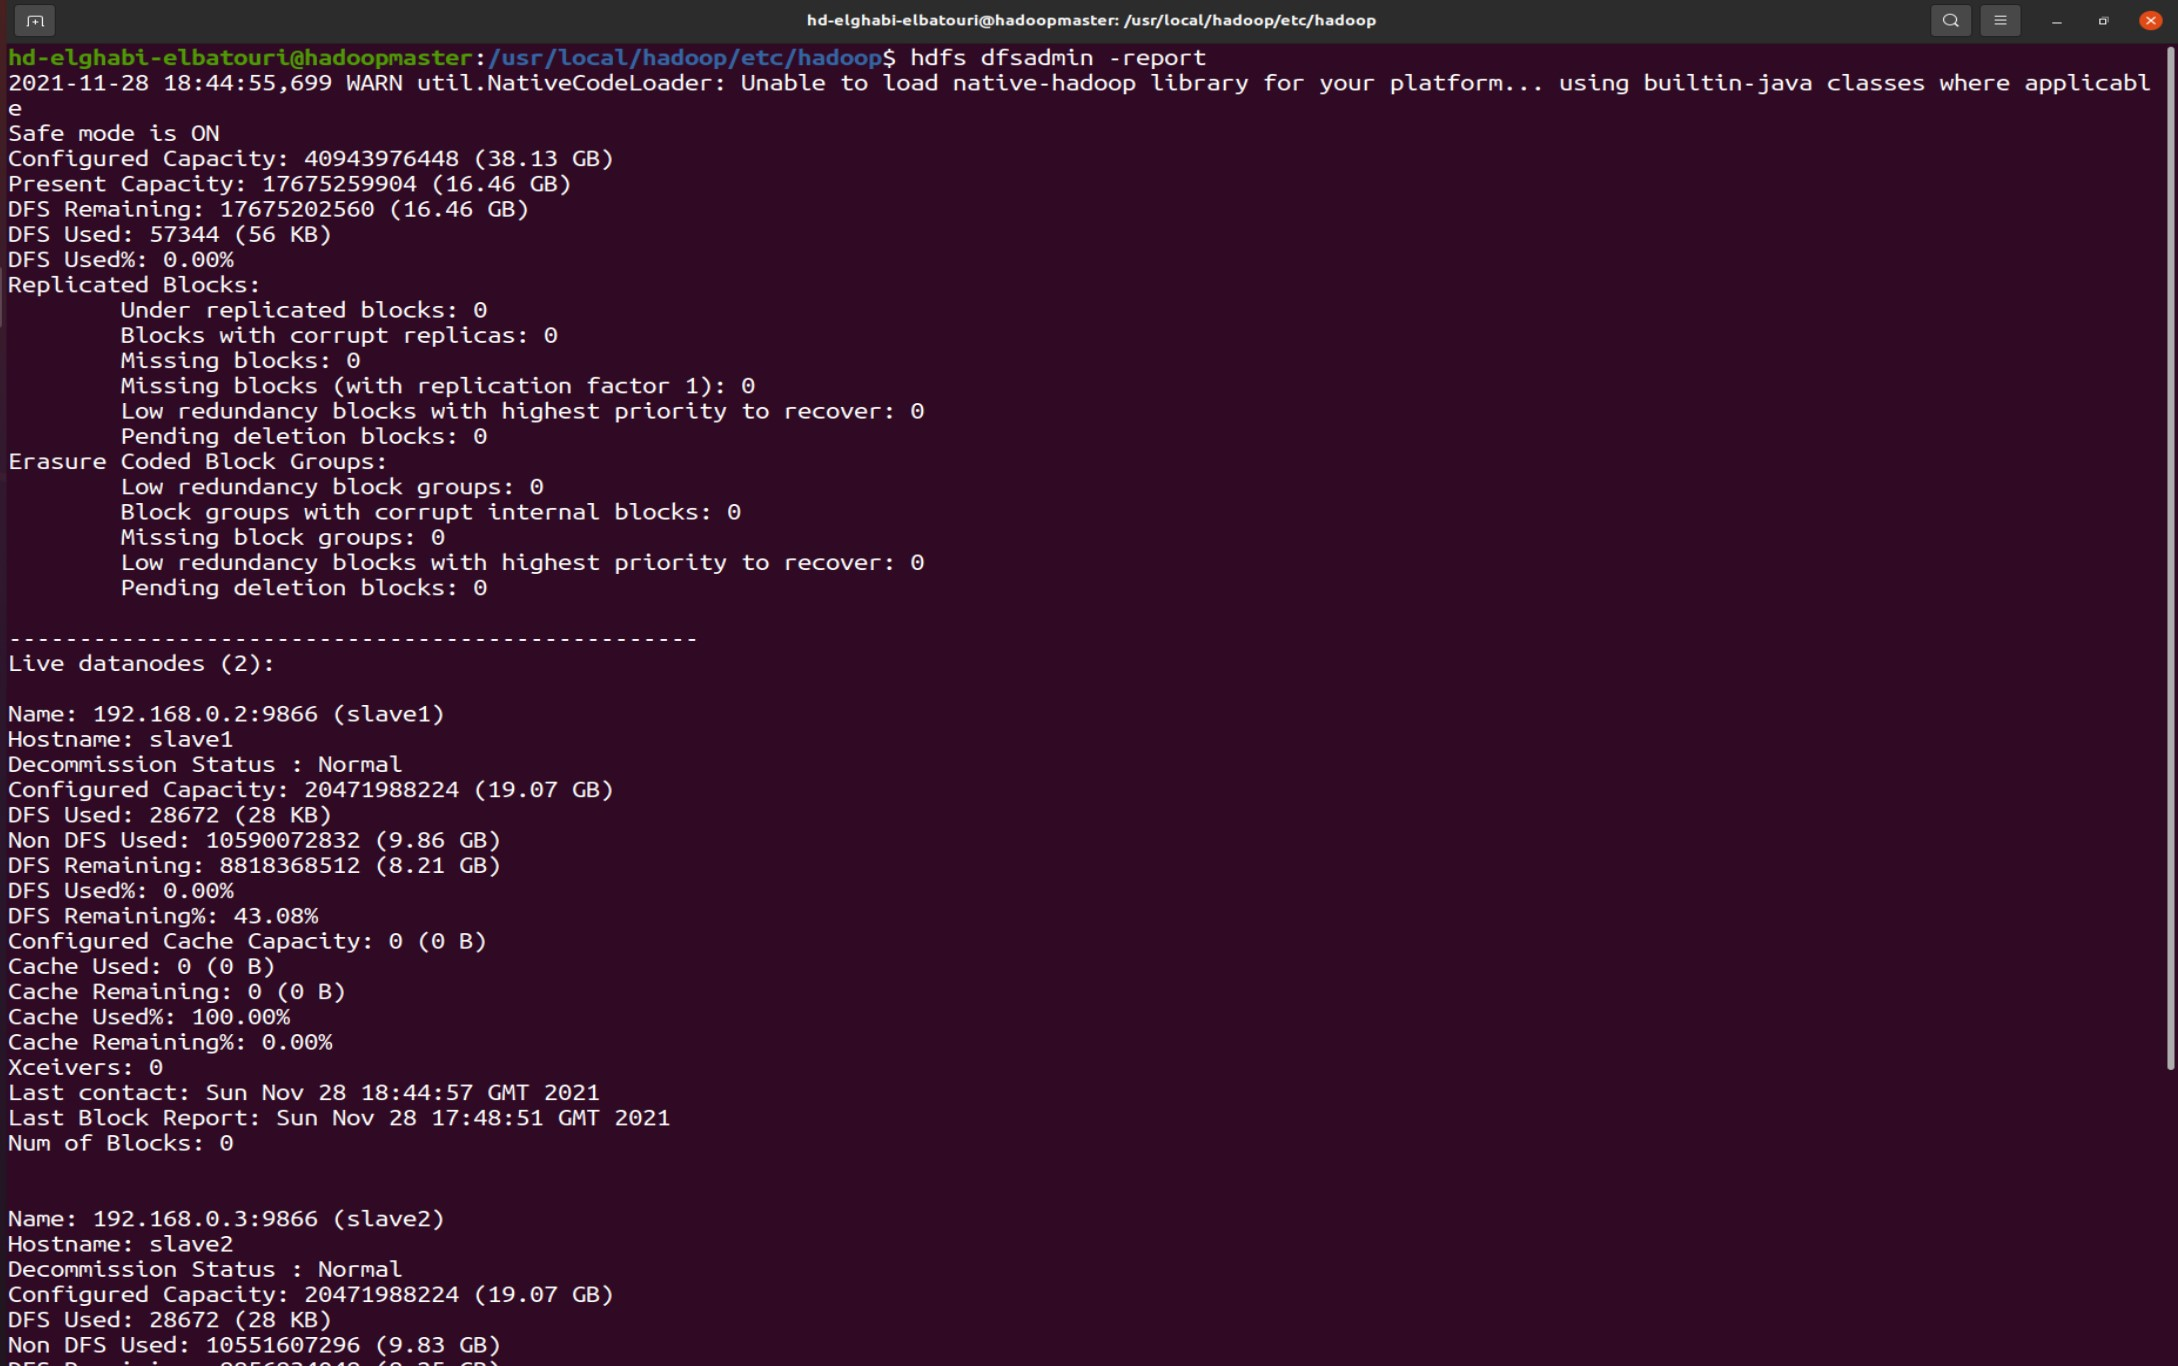
\includegraphics[width=1\linewidth]{Big_Data/Hadoop/Multi-Nodes Map_Reduce/Verifying cluster nodes.jpg} 
\end{center} 
\caption{caption} 
\end{figure} 
\FloatBarrier



\section{Executing Map/Reduce}

\par thisIsAveryLongParagraphToUseAsAtemplateForCopyAndPastingContentInAgoodWay
\\
\begin{figure}[!htb] 
\begin{center} 
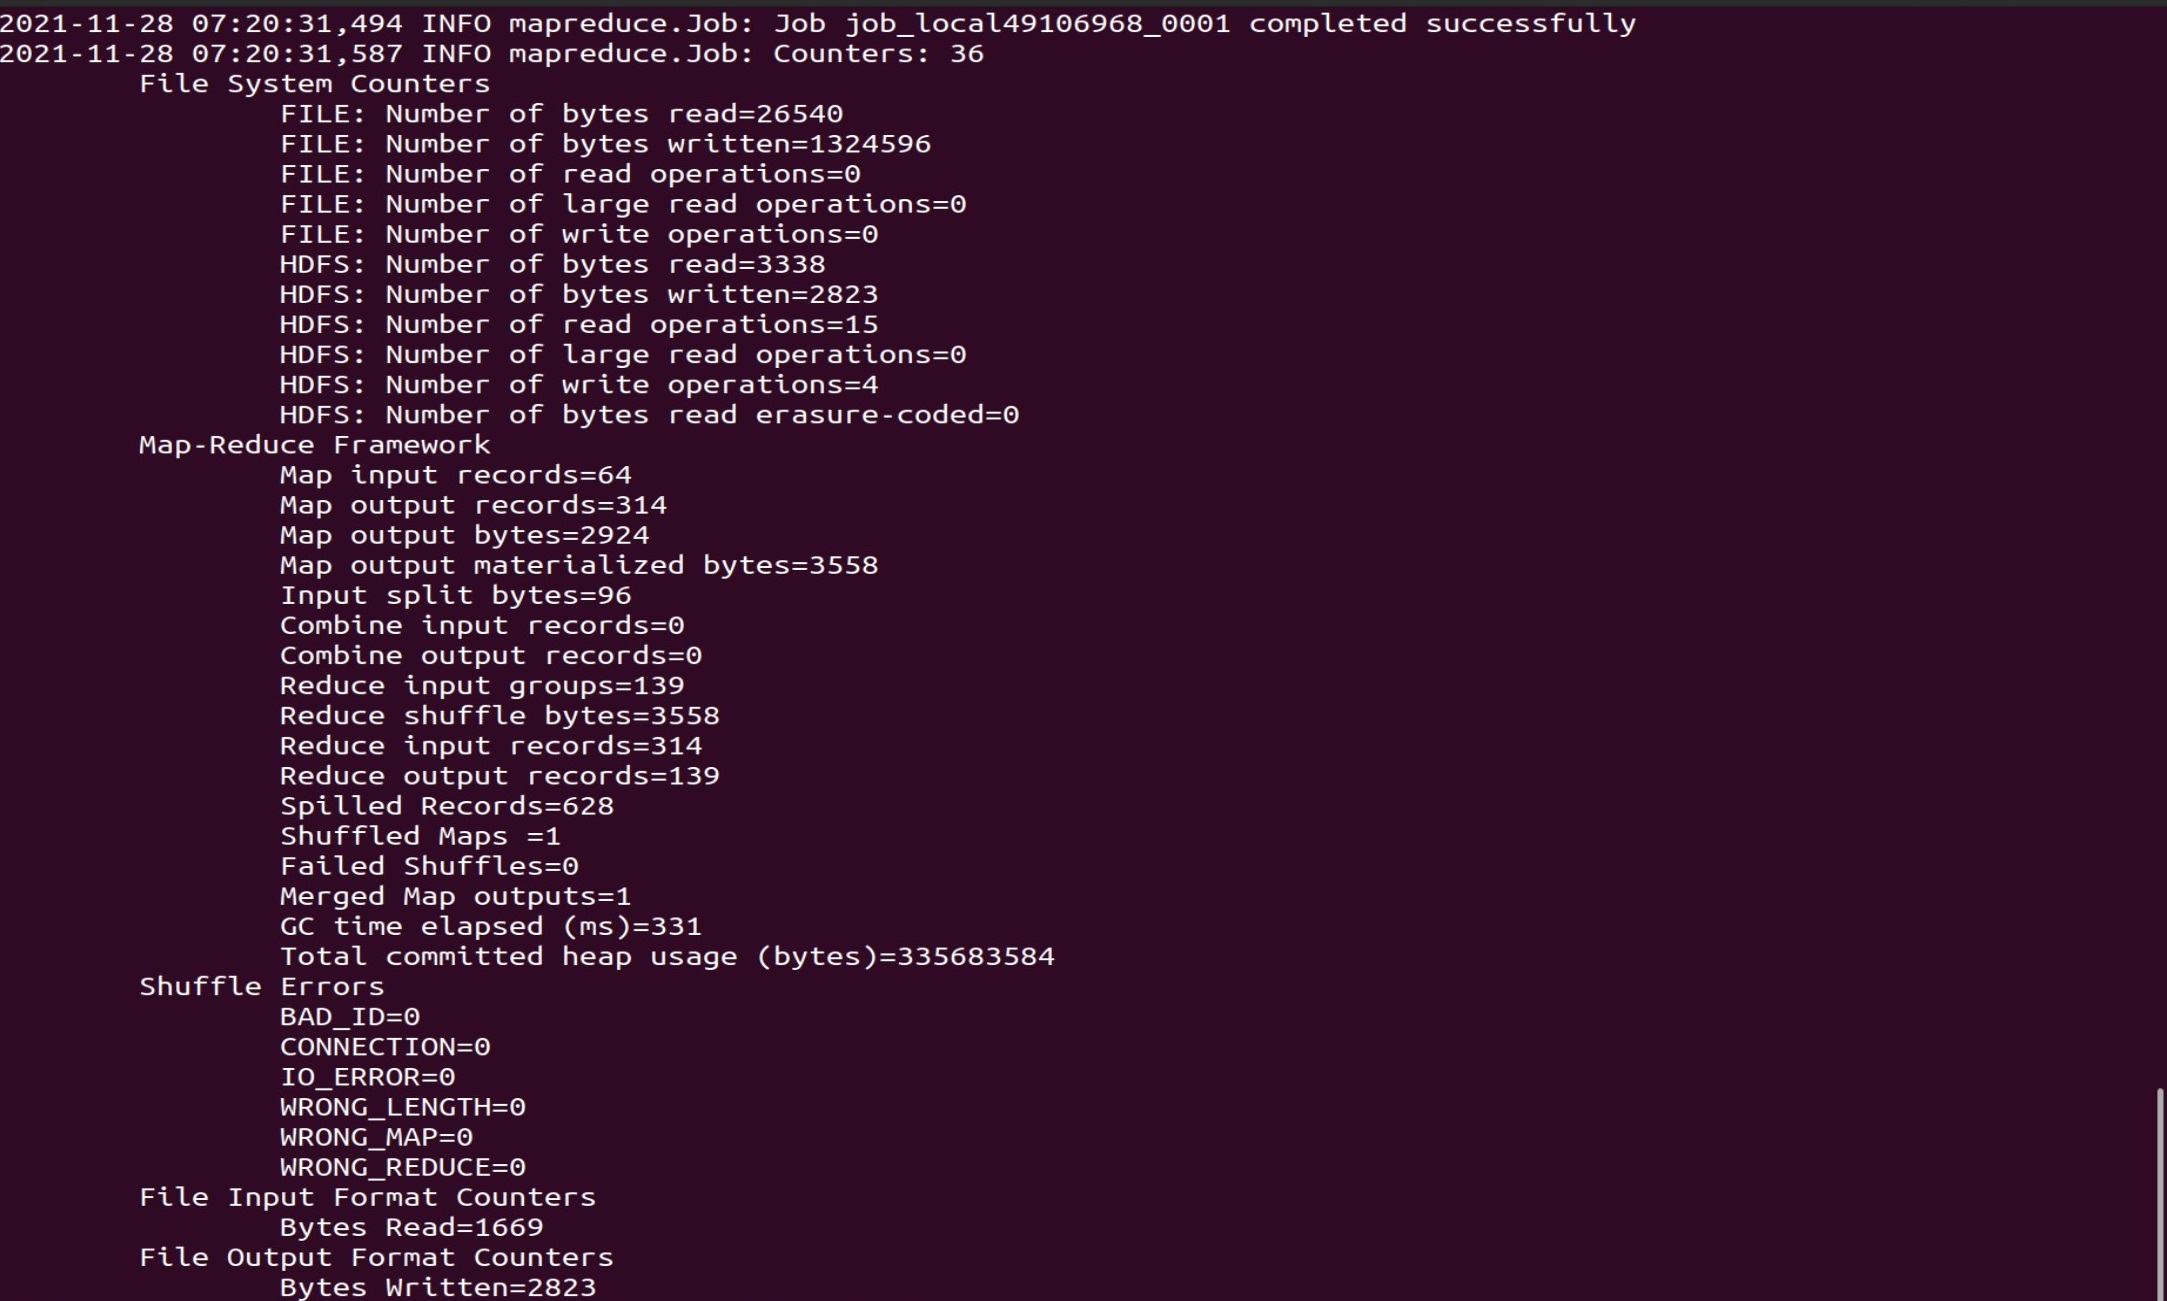
\includegraphics[width=1\linewidth]{Big_Data/Hadoop/Multi-Nodes Map_Reduce/running wordcount.jpg} 
\end{center} 
\caption{caption} 
\end{figure} 
\FloatBarrier


\section{Showing results}

\par Getting the result of the Map / Reduce algorithm.
\\
\begin{figure}[!htb] 
\begin{center} 
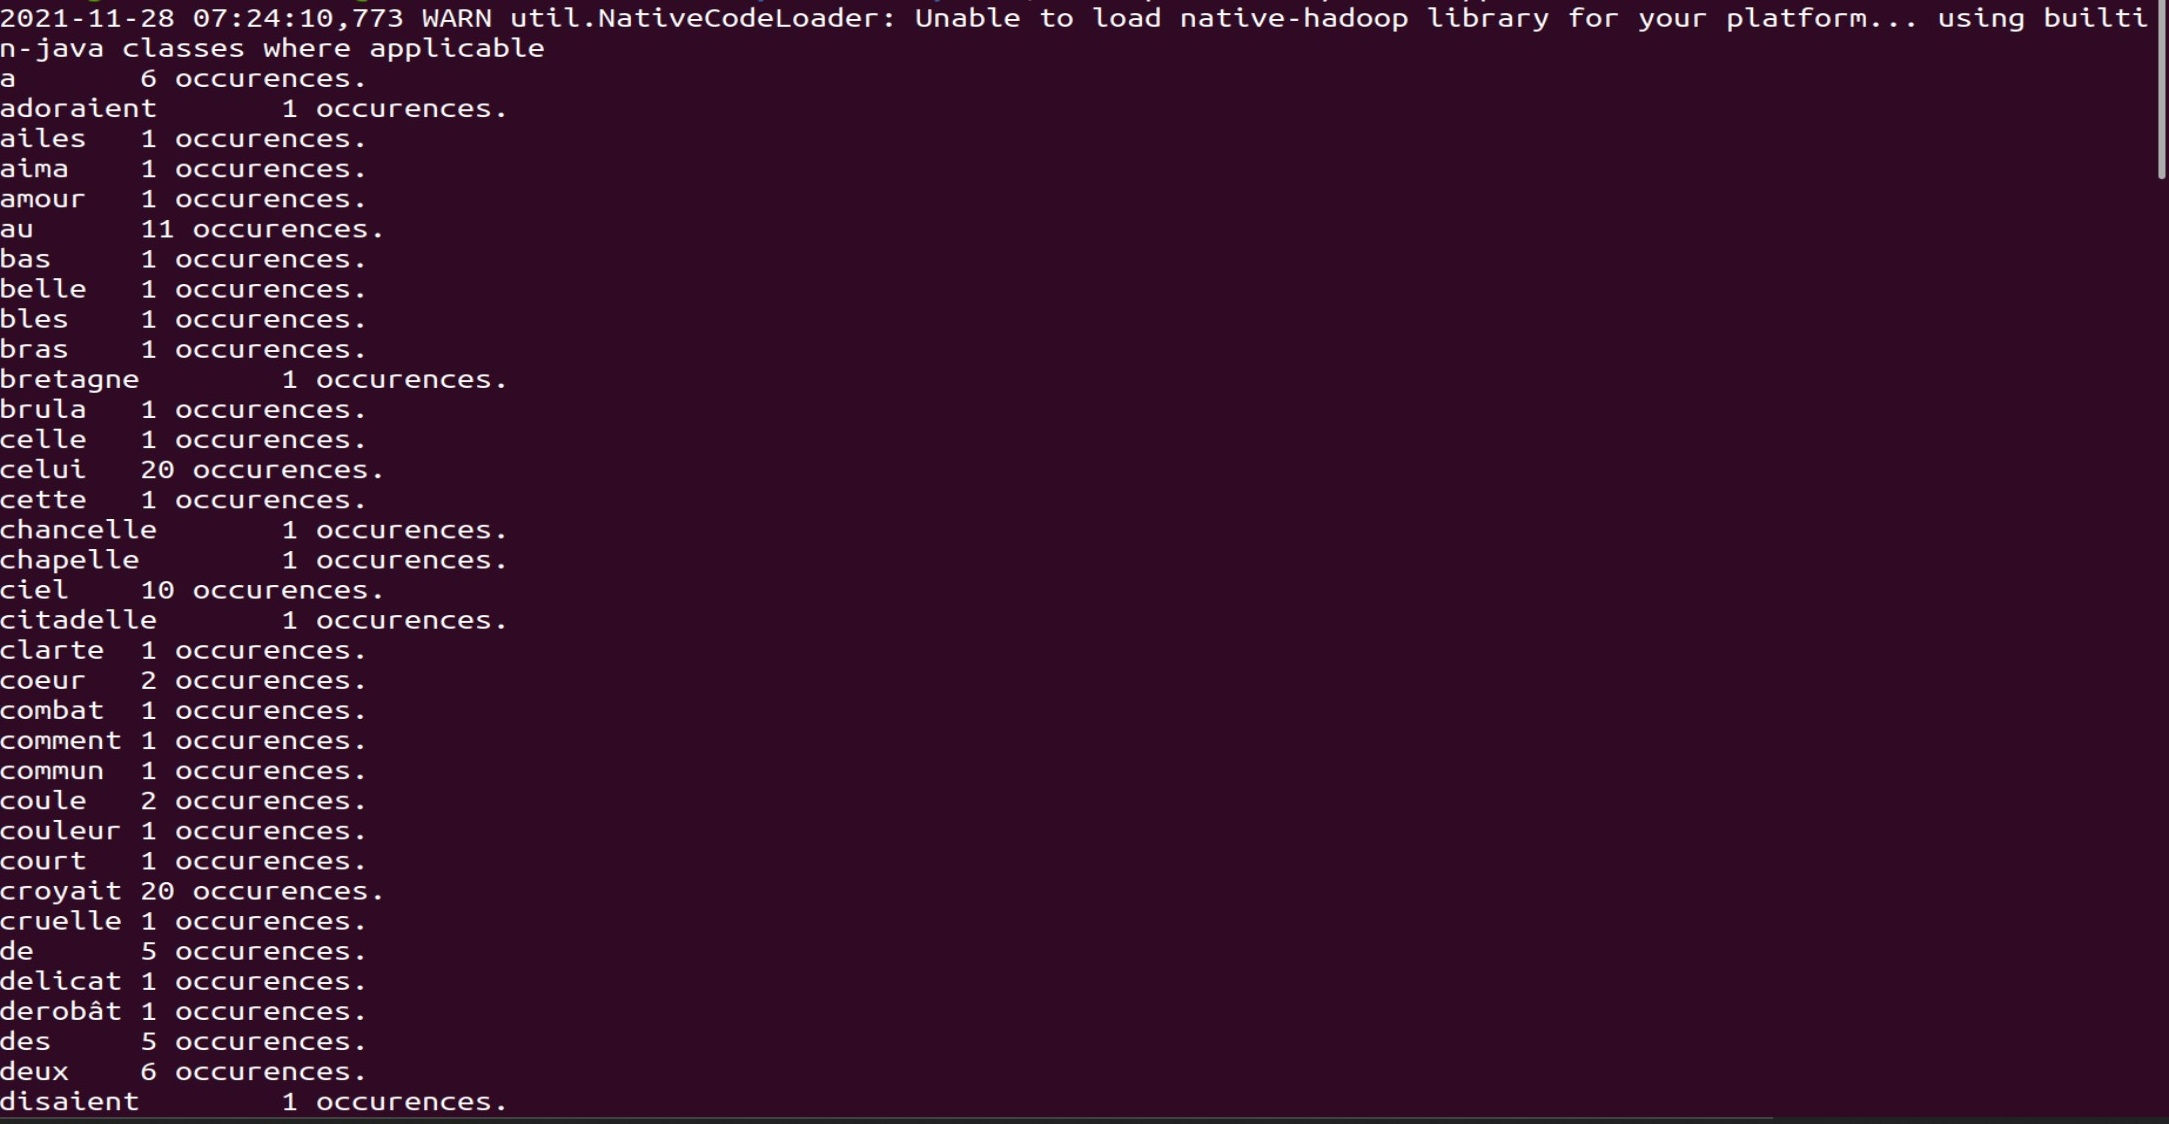
\includegraphics[width=1\linewidth]{Big_Data/Hadoop/Multi-Nodes Map_Reduce/Showing results.jpg} 
\end{center} 
\caption{caption} 
\end{figure} 
\FloatBarrier


\end{spacing}